\documentclass[10pt,a4paper]{article}
\usepackage[margin=1in]{geometry}
\usepackage{lmodern}        % scalable Type-1 Computer Modern (microtype needs it)
\usepackage{graphicx}
\usepackage{booktabs}
\usepackage{xcolor}
\usepackage{hyperref}
\usepackage{microtype}
\usepackage{caption}
\usepackage{titling}
\usepackage{authblk}
\usepackage{orcidlink}

\hypersetup{
  colorlinks=true,
  linkcolor=blue!50!black,
  citecolor=blue!50!black,
  urlcolor=blue!50!black,
}

\setlength{\droptitle}{-3em}

\title{\Large Backend Performance Asymmetries on AMD Strix Halo \\
       for LLM Inference: \\
       \large A Case Study of ROCm/HIP vs.\ Mesa RADV Vulkan on gfx1151}

\author[1]{Paul Durkin\thanks{paul@northstaraurora.ai}\,\orcidlink{0009-0000-2537-1578}}
\affil[1]{NorthStar Aurora}

\date{\today}

\begin{document}
\maketitle

\begin{abstract}
The AMD Strix Halo platform (Ryzen AI MAX+ 395 with a Radeon 8060S iGPU on the gfx1151 RDNA 3.5 ISA and 128~GiB of unified memory) offers an unusual combination for solo LLM developers: enough VRAM to load 27--35B-parameter models without quantization, at approximately one third of the cost of an equivalent NVIDIA-class workstation. The hardware ships with two viable GPU inference backends in \texttt{llama.cpp}: AMD's official ROCm/HIP stack, and Mesa's open-source RADV Vulkan driver with cooperative-matrix support. We benchmark both at an identical source commit on the Qwen3.6-35B-A3B model and find a precision-dependent asymmetry: Vulkan outperforms ROCm by 19--22\% on Q4\_K\_M decode, while ROCm outperforms Vulkan by 117--121\% on BF16 decode. The asymmetry is attributable to a single missing capability (\texttt{bf16:0}) in the Mesa STRIX\_HALO Vulkan driver. Separately, we show that \texttt{GGML\_HIP\_ROCWMMA\_FATTN=OFF}---a flag that AMD's published RDNA 3.5 best-practices recommends enabling---in fact yields up to 145\% higher prefill throughput at 8K context on gfx1151. We release the full benchmark dataset and reproduction recipes under MIT.

\textbf{Keywords:} LLM inference, AMD Strix Halo, gfx1151, ROCm, HIP, Vulkan, Mesa RADV, llama.cpp, BF16, flash attention.
\end{abstract}

\section{Introduction}

The economics of fine-tuning and serving large language models on a single workstation have shifted with the introduction of consumer AMD APUs that pair Zen 5 CPU cores with an RDNA 3.5 iGPU on a shared 128~GiB LPDDR5x pool. The AMD Strix Halo platform (Ryzen AI MAX+ 395), packaged in workstations such as the Corsair AI Workstation 300 at approximately \$2,400, can hold a fully-precision (BF16) 27B-parameter model entirely in unified memory---a workload that on NVIDIA would require an H100 (80~GiB HBM3) at roughly 8--10$\times$ the cost.

This price/capacity ratio has driven a wave of community interest in Strix Halo as a solo-developer LLM platform, but the software stack remains immature in places where production decisions must be made. In particular, the \texttt{llama.cpp} inference engine~\cite{llamacpp} supports two GPU backends that compile from the same source tree:

\begin{itemize}
  \item \textbf{ROCm/HIP}---AMD's official compute stack. Built with \texttt{-DGGML\_HIP=ON}, links against \texttt{libamdhip64}. The only path that interoperates with PyTorch nightly for training.
  \item \textbf{Vulkan via Mesa RADV}---the open-source graphics driver path. Built with \texttt{-DGGML\_VULKAN=ON}, links against \texttt{libvulkan}. Mesa 25.x added explicit STRIX\_HALO support; recent kernels expose the compute features needed by the cooperative-matrix code path.
\end{itemize}

Public benchmark dashboards (notably bench.ciru.ai) report markedly higher Vulkan throughput for quantized models, while our own production deployment ran ROCm exclusively (training forces the choice). The discrepancy prompted a head-to-head comparison at an identical source commit. The result was not a one-way win: instead we found a precision-boundary asymmetry that, to our knowledge, has not been quantified in the literature.

This paper makes three concrete contributions:

\begin{enumerate}
  \item \textbf{Quantification of the ROCm/Vulkan precision inversion on gfx1151.} On Qwen3.6-35B-A3B (Section~\ref{sec:results-vrocm}), Vulkan/RADV wins decode by approximately 22\% at Q4\_K\_M, while ROCm/HIP wins decode by approximately 117\% (\(\sim 2.2\times\)) at BF16. The crossover is driven by a single missing capability in Mesa's STRIX\_HALO Vulkan driver, visible in its own startup log.
  \item \textbf{Empirical contradiction of AMD's RDNA 3.5 best-practices for flash attention.} The vendor's published optimization guide~\cite{amdrdna35} recommends enabling \texttt{GGML\_HIP\_ROCWMMA\_FATTN}. We show (Section~\ref{sec:results-rocwmma}) that disabling it improves prefill throughput by 14--145\% across context depths on both a dense Qwen3.5-27B Q8 model and a MoE Qwen3.6-35B-A3B Q4 model.
  \item \textbf{Public release of the benchmark dataset.} All raw \texttt{llama.cpp} bench logs, build scripts, and reproduction recipes are available under MIT at the Hugging Face dataset \texttt{NorthstarAurora/strix-halo-bench-data}~\cite{benchdata}, the long-form writeup~\cite{longform}, and the production guide repository~\cite{guide}.
\end{enumerate}

\section{Background}

The AMD Strix Halo SoC integrates a 16-core Zen~5/Zen~5c CPU complex with a Radeon~8060S iGPU exposing 40 RDNA~3.5 compute units. The defining characteristic for LLM workloads is the shared memory architecture: there is no dedicated VRAM. The full 128~GiB system pool is addressable as GPU memory via the kernel's GTT auto-sizing, with the BIOS UMA region typically configured to its minimum (1~GiB) and the kernel handling allocation dynamically through the amdgpu driver.

On the software side, \texttt{llama.cpp} dispatches GPU operations through pluggable backends. The HIP backend (\texttt{libggml-hip.so}) translates ggml operations into HIP kernels, which then dispatch to AMD's matrix and shader hardware through \texttt{libamdhip64}. The Vulkan backend (\texttt{libggml-vulkan.so}) uses the Vulkan compute API; on AMD hardware the Mesa RADV driver translates Vulkan SPIR-V into hardware shaders, optionally using the cooperative-matrix extensions for tensor-class operations.

Cooperative matrix is the Vulkan equivalent of CUDA's tensor cores or HIP's WMMA intrinsics: a small fixed-size matrix multiply primitive that maps to dedicated hardware. The \texttt{VK\_KHR\_cooperative\_matrix} extension specifies which numeric types (FP16, FP32, BF16, INT8, etc.) the driver supports for these primitives. A driver may support fewer types than the hardware physically implements, particularly for newer types where the driver's lowering passes have not yet been written.

\section{Methodology}\label{sec:methodology}

\subsection{Test rig}

All measurements were taken on a single workstation:

\begin{itemize}
  \item \textbf{CPU/GPU:} AMD Ryzen AI MAX+ 395 with Radeon 8060S iGPU (gfx1151, RDNA 3.5, 40 CUs)
  \item \textbf{Memory:} 128~GiB LPDDR5x-8000 unified pool; BIOS UMA 1~GiB; kernel GTT auto-sized to the full 128~GiB
  \item \textbf{OS:} Ubuntu 24.04 LTS, kernel 6.19.14 mainline (KFD + amdgpu fence/dma\_buf fixes for gfx1151)
  \item \textbf{ROCm:} 7.1.0 system install + nightly \texttt{libhsa-runtime64.so.1} overlay from PyTorch's \texttt{\_rocm\_sdk\_core} wheel (required to dodge a null-pointer bug in 7.1.0 stock HSA on gfx1151)
  \item \textbf{Mesa:} 25.2.8 (RADV STRIX\_HALO support built in)
\end{itemize}

\subsection{Build configuration}

Both backends were compiled from \texttt{ggerganov/llama.cpp} commit \texttt{a497476} (release tag \texttt{b9296}).

The HIP build used the flag set recommended by the strix-halo-llm-finetune-guide~\cite{guide}:
\begin{verbatim}
-DGGML_HIP=ON -DGGML_HIP_ROCWMMA_FATTN=OFF
-DGGML_HIP_MMQ_MFMA=ON -DGGML_HIP_NO_VMM=ON
-DGGML_HIP_GRAPHS=ON -DAMDGPU_TARGETS=gfx1151
-DCMAKE_HIP_FLAGS='--gcc-install-dir=/usr/lib/gcc/x86_64-linux-gnu/13'
\end{verbatim}
\noindent The \texttt{--gcc-install-dir} flag is required on Ubuntu 24.04 to prevent ROCm 7.1's clang-20 from picking the gcc-14 runtime directory, which lacks the C++ standard headers (\texttt{<cmath>}, \texttt{<cstdlib>}).

The Vulkan build used \texttt{-DGGML\_VULKAN=ON -DGGML\_NATIVE=ON} with no HIP libraries linked.

\subsection{Bench protocol}

\texttt{llama-bench} was invoked identically against both backends for two shape configurations:
\begin{verbatim}
-p 512  -n 128 -r 3 --mmap 0 -ngl 99 -fa 0,1
-p 2048 -n 128 -r 3 --mmap 0 -ngl 99 -fa 1 -d 0,4196,8392
\end{verbatim}
\noindent Three repetitions per cell; standard deviation reported. The \texttt{--mmap 0} flag is critical on Strix Halo: mmap-only model loading triggers a 30-minute GPU page-table setup, undocumented but reproducible (see~\cite{guide}, Step 7a). The depth sweep at \texttt{-d 0,4196,8392} exercises the KV-cache scaling path that is the dominant cost for real chat workloads beyond the trivial-context case.

For the ROCm runs the launch environment included \texttt{LD\_LIBRARY\_PATH=\$NIGHTLY\_LIB:/opt/rocm-7.1.0/lib} where \texttt{\$NIGHTLY\_LIB} is the PyTorch \texttt{\_rocm\_sdk\_core} overlay directory. Vulkan needed no overlay---Mesa is the driver.

Model files were the public Unsloth GGUF releases: \texttt{unsloth/Qwen3.6-35B-A3B-GGUF} at Q4\_K\_M (UD variant, 20.6~GiB) and BF16 (66~GiB), and \texttt{unsloth/Qwen3.5-27B-Instruct-GGUF} at Q8\_0 (26.6~GiB).

\section{Results: ROCm/HIP vs.\ Mesa RADV Vulkan}\label{sec:results-vrocm}

\subsection{Quantized inference (Q4\_K\_M)}

For the Q4\_K\_M variant of Qwen3.6-35B-A3B, Vulkan outperforms ROCm on decode at every context depth measured, by a consistent 19--22\% margin (Figure~\ref{fig:q4}, Table~\ref{tab:q4}). Prefill at shallow context favors ROCm by approximately 7\%, but the gap closes by 8K tokens and Vulkan slightly leads at d=8392.

\begin{figure}[h]
  \centering
  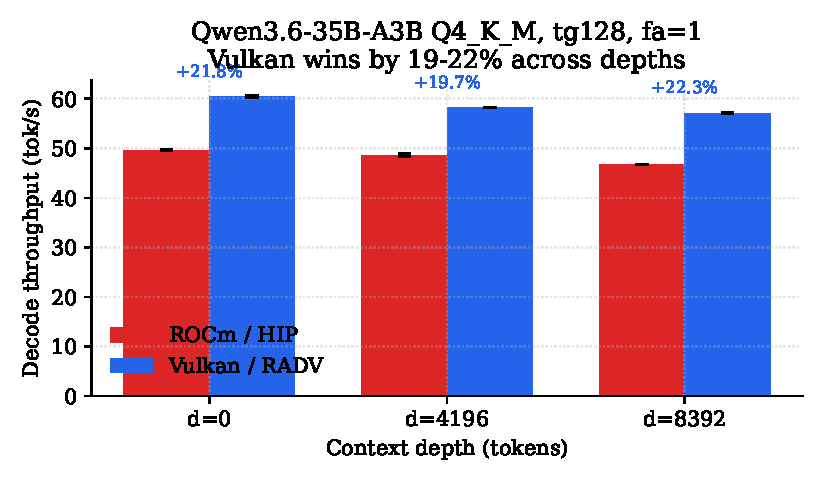
\includegraphics[width=0.85\linewidth]{figures/fig1-vulkan-vs-rocm-q4.pdf}
  \caption{Decode throughput on Qwen3.6-35B-A3B Q4\_K\_M, tg128 at fa=1, across context depths. Vulkan/RADV outperforms ROCm/HIP by approximately 22\% consistently. Three runs per cell; error bars show one standard deviation.}
  \label{fig:q4}
\end{figure}

\begin{table}[h]
\centering
\small
\begin{tabular}{lrrr}
\toprule
shape & ROCm/HIP & Vulkan & winner \\
\midrule
pp512 fa=0          & 1023.75 $\pm$ 8.66 & 953.79 $\pm$ 17.18 & ROCm +7.3\% \\
pp512 fa=1          & 1014.32 $\pm$ 9.65 & 942.18 $\pm$ 4.92 & ROCm +7.7\% \\
\textbf{tg128 d=0 fa=1}     & 49.58 $\pm$ 0.09 & \textbf{60.39 $\pm$ 0.22} & \textbf{Vulkan +21.8\%} \\
\textbf{tg128 d=4196 fa=1}  & 48.64 $\pm$ 0.24 & \textbf{58.24 $\pm$ 0.09} & \textbf{Vulkan +19.7\%} \\
\textbf{tg128 d=8392 fa=1}  & 46.73 $\pm$ 0.02 & \textbf{57.13 $\pm$ 0.09} & \textbf{Vulkan +22.3\%} \\
pp2048 d=0 fa=1     & 983.86 $\pm$ 2.91 & 921.04 $\pm$ 2.97 & ROCm +6.8\% \\
pp2048 d=8392 fa=1  & 815.70 $\pm$ 0.57 & 835.33 $\pm$ 2.28 & Vulkan +2.4\% \\
\bottomrule
\end{tabular}
\caption{Qwen3.6-35B-A3B Q4\_K\_M throughput, tok/s, 3 reps. Vulkan dominates decode; ROCm has a small prefill edge that closes by deep context.}
\label{tab:q4}
\end{table}

\subsection{Full-precision inference (BF16)}

The BF16 run inverts the picture (Figure~\ref{fig:bf16}, Table~\ref{tab:bf16}). ROCm outperforms Vulkan by 117--121\% on decode---over a factor of two---and by 51--59\% on prefill, on the same model, same source commit, same hardware. The only meaningful difference is the GGUF precision.

\begin{figure}[h]
  \centering
  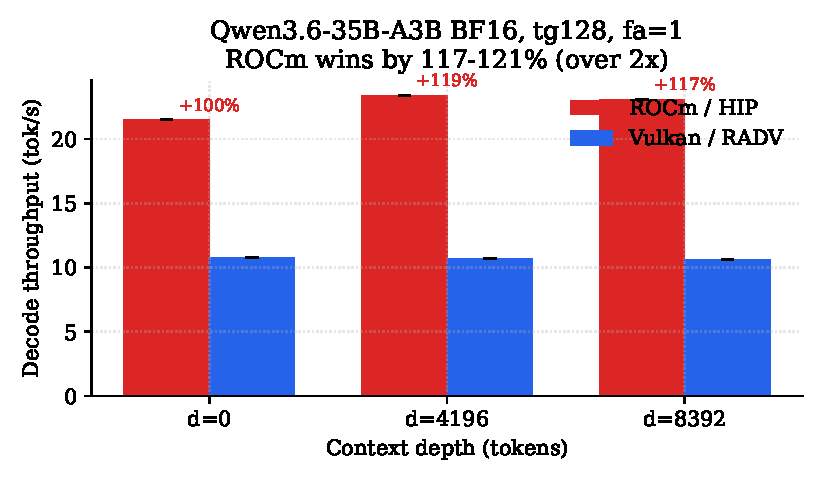
\includegraphics[width=0.85\linewidth]{figures/fig2-vulkan-vs-rocm-bf16.pdf}
  \caption{Decode throughput on Qwen3.6-35B-A3B BF16, tg128 at fa=1. ROCm/HIP outperforms Vulkan/RADV by approximately 117--121\% across depths. The relative ordering inverts versus Figure~\ref{fig:q4}.}
  \label{fig:bf16}
\end{figure}

\begin{table}[h]
\centering
\small
\begin{tabular}{lrrr}
\toprule
shape & ROCm/HIP & Vulkan & winner \\
\midrule
\textbf{pp512 fa=0}         & \textbf{479.55 $\pm$ 1.69} & 306.85 $\pm$ 1.00 & \textbf{ROCm +56.3\%} \\
\textbf{pp512 fa=1}         & \textbf{484.01 $\pm$ 4.40} & 305.21 $\pm$ 0.87 & \textbf{ROCm +58.6\%} \\
\textbf{tg128 d=0 fa=1}     & \textbf{23.71 $\pm$ 0.01} & 10.73 $\pm$ 0.00 & \textbf{ROCm +121\%} \\
\textbf{tg128 d=4196 fa=1}  & \textbf{23.39 $\pm$ 0.01} & 10.68 $\pm$ 0.01 & \textbf{ROCm +119\%} \\
\textbf{tg128 d=8392 fa=1}  & \textbf{23.09 $\pm$ 0.00} & 10.64 $\pm$ 0.00 & \textbf{ROCm +117\%} \\
\textbf{pp2048 d=0 fa=1}    & \textbf{474.69 $\pm$ 2.76} & 307.44 $\pm$ 1.28 & \textbf{ROCm +54.4\%} \\
\textbf{pp2048 d=8392 fa=1} & \textbf{440.02 $\pm$ 0.67} & 289.64 $\pm$ 0.84 & \textbf{ROCm +51.9\%} \\
\bottomrule
\end{tabular}
\caption{Qwen3.6-35B-A3B BF16 throughput, tok/s, 3 reps. ROCm wins everything by 50--120\%; the magnitudes are large and stable.}
\label{tab:bf16}
\end{table}

\subsection{Root cause: \texttt{bf16:0} on RADV STRIX\_HALO}

The Vulkan backend's startup log on this hardware emits its driver capability summary:

\begin{small}
\begin{verbatim}
ggml_vulkan: 0 = AMD Radeon Graphics (RADV GFX1151) (radv) |
  uma: 1 | fp16: 1 | bf16: 0 | warp size: 64 | shared memory: 65536 |
  int dot: 0 | matrix cores: KHR_coopmat
\end{verbatim}
\end{small}

\noindent\texttt{fp16: 1} indicates that the cooperative-matrix path supports FP16 inputs; \texttt{bf16: 0} indicates it does not support BF16. When a BF16 model is loaded, the ggml-vulkan backend falls back from the cooperative-matrix primitive to general-purpose shader code (FP32 emulation, in practice) for matmul operations. The same hardware executes FP16 matmul at full rate but processes BF16 in software.

ROCm/HIP does not have this gap: \texttt{libggml-hip.so} dispatches BF16 matmul through HIP kernels that target the same matrix units the RADV path lacks coverage for. On the BF16 path, the two backends are therefore performing fundamentally different work on identical silicon.

This is a Mesa-side gap, not a llama.cpp gap. Cooperative-matrix BF16 extensions for RADV STRIX\_HALO are tracked work-in-progress~\cite{vkcoopmat2}; once the lowering passes land in Mesa, the Vulkan BF16 numbers should improve substantially and the inversion may disappear.

\section{Results: \texttt{GGML\_HIP\_ROCWMMA\_FATTN} Toggle}\label{sec:results-rocwmma}

AMD's official RDNA 3.5 best-practices document~\cite{amdrdna35} recommends building llama.cpp with \texttt{GGML\_HIP\_ROCWMMA\_FATTN=ON} on consumer AMD GPUs for ``faster flash-attention.'' On gfx1151 specifically we find the opposite (Figure~\ref{fig:fattn}, Table~\ref{tab:fattn}): the flag should be \emph{disabled}, by margins ranging from minor (zero on decode) to dramatic (145\% on prefill at 8K context).

\begin{figure}[h]
  \centering
  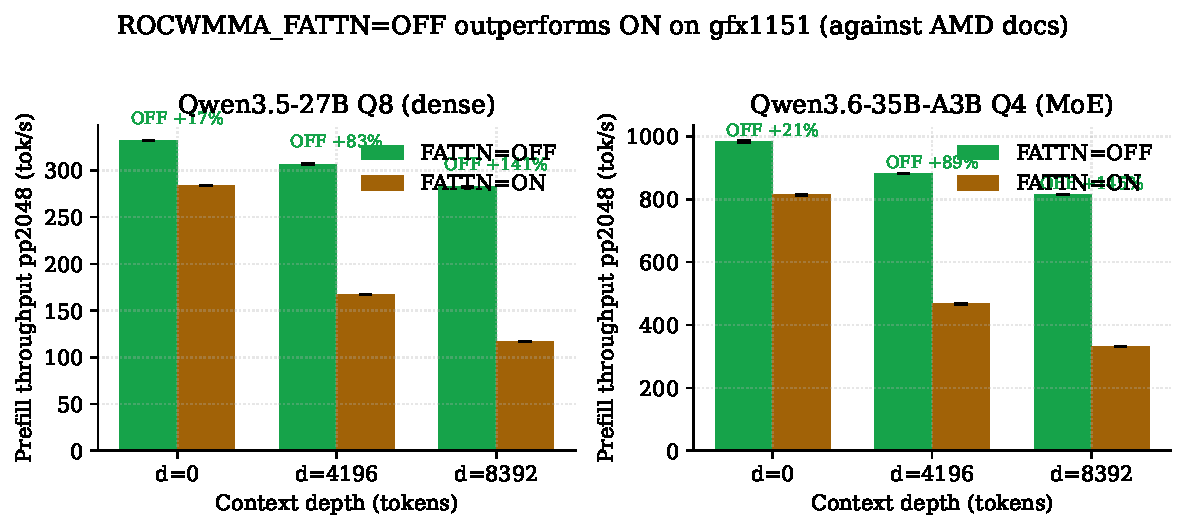
\includegraphics[width=0.95\linewidth]{figures/fig3-rocwmma-fattn-onoff.pdf}
  \caption{Prefill throughput pp2048 on two models, three context depths, with \texttt{GGML\_HIP\_ROCWMMA\_FATTN=OFF} vs.\ ON. OFF consistently wins; the gap widens at deeper context. Both the dense Qwen3.5-27B Q8 model and the MoE Qwen3.6-35B-A3B Q4 model show the same pattern.}
  \label{fig:fattn}
\end{figure}

\begin{table}[h]
\centering
\small
\begin{tabular}{llrrr}
\toprule
model & shape & OFF & ON & winner \\
\midrule
Qwen3.5-27B Q8 (dense)  & pp2048 d=0    & 331.86 $\pm$ 0.06 & 264.36 $\pm$ 5.99 & OFF +25.5\% \\
Qwen3.5-27B Q8 (dense)  & pp2048 d=4196 & 306.83 $\pm$ 0.45 & 173.96 $\pm$ 0.81 & OFF +76.4\% \\
\textbf{Qwen3.5-27B Q8} & \textbf{pp2048 d=8392} & \textbf{282.52 $\pm$ 0.52} & \textbf{117.08 $\pm$ 1.83} & \textbf{OFF +141\%} \\
\midrule
Qwen3.6-35B-A3B Q4 (MoE) & pp2048 d=0    & 983.86 $\pm$ 2.91 & 814.66 $\pm$ 6.78 & OFF +20.8\% \\
Qwen3.6-35B-A3B Q4 (MoE) & pp2048 d=4196 & 873.20 $\pm$ 0.92 & 461.92 $\pm$ 2.05 & OFF +89.0\% \\
\textbf{Qwen3.6-35B-A3B Q4} & \textbf{pp2048 d=8392} & \textbf{815.70 $\pm$ 0.57} & \textbf{333.13 $\pm$ 1.36} & \textbf{OFF +145\%} \\
\midrule
\multicolumn{2}{l}{tg128 (any model/depth)} & \multicolumn{3}{c}{statistically tied, no effect} \\
\bottomrule
\end{tabular}
\caption{ROCWMMA\_FATTN ON vs.\ OFF, pp2048 throughput, tok/s. The decode (tg128) path is memory-bandwidth bound and the toggle does not affect it; the entire effect is on the prefill (compute-bound) path, where it gets dramatic at deep context.}
\label{tab:fattn}
\end{table}

The Unsloth Studio installer~\cite{unsloth} and the lemonade-sdk pre-built llama.cpp~\cite{lemonade} both already default to \texttt{ROCWMMA\_FATTN=OFF}, so the practical impact on those installation paths is zero. Users who build llama.cpp from source against AMD's own documentation, however, would silently lose 1.4--2.4$\times$ prefill throughput at the context depths where the gap matters most.

\section{Discussion}

\subsection{Practical guidance}

The two findings combine to a simple decision matrix for solo developers on Strix Halo:

\begin{itemize}
  \item \textbf{Quantized inference} (Q4--Q8): use Mesa RADV Vulkan. The decode throughput advantage is large (\(\sim\)22\%), consistent across depths, and the prefill cost is small. The bench.ciru.ai dashboard~\cite{benchciru} is the canonical reference for Vulkan numbers in this regime.
  \item \textbf{Full-precision (BF16) inference}: use ROCm/HIP. The decode throughput advantage is \(\sim\)2.2\(\times\) and the prefill advantage is \(\sim\)55\%---both dominant.
  \item \textbf{Training}: ROCm is forced (PyTorch nightly + ROCm 7.13 is the only working path). Training is BF16, so the choice aligns with the BF16 inference recommendation.
  \item \textbf{Mixed workloads}: pin the inference side to whichever backend matches the hot path. Source-built llama.cpp should set \texttt{ROCWMMA\_FATTN=OFF} regardless.
\end{itemize}

\subsection{Limitations}

\begin{itemize}
  \item \textbf{Single hardware platform.} All measurements are from one Strix Halo workstation. The findings are silicon-specific: the \texttt{bf16:0} gap is a Mesa STRIX\_HALO codepath limitation that may differ on RDNA 3 discrete cards (RX 7900) or RDNA 4 (RX 9070 XT) which use different Vulkan capability profiles. Similarly the ROCWMMA\_FATTN observation may not generalize off gfx1151.
  \item \textbf{Model coverage.} We tested two model architectures: dense (Qwen3.5-27B) and MoE (Qwen3.6-35B-A3B). The trends are consistent across both but a fuller architecture sweep (recurrent, vision, audio) would strengthen the generality claim.
  \item \textbf{Temporal scope.} Both Mesa and AMD ROCm are under active development; the numbers reported here are accurate as of Mesa 25.2.8 and ROCm 7.1.0 (with the 7.13 HSA overlay) but the gap is expected to close as Mesa's BF16 cooperative-matrix support lands.
  \item \textbf{Bench shape.} \texttt{llama-bench} measures isolated forward passes; production serving overhead (KV-cache management, batching, scheduling) is not modeled here.
\end{itemize}

\subsection{Implications for vendor documentation}

The ROCWMMA\_FATTN finding suggests that AMD's published RDNA 3.5 best-practices document should be updated, at least with respect to the gfx1151 configuration. The current recommendation produces measurable performance regressions in the very workload (long-context LLM inference) it is intended to optimize. We have not yet investigated whether the recommendation is correct for discrete RDNA 3 / 3.5 cards, where the underlying matrix units may behave differently.

\section{Related Work}

This work intersects with several existing communities. The \texttt{llama.cpp} project~\cite{llamacpp} has accumulated a body of empirical micro-benchmarks in its issues and discussions, but precision-asymmetry on AMD APUs specifically does not appear in the indexed material we surveyed. The bench.ciru.ai dashboard~\cite{benchciru} provides excellent Vulkan-only Strix Halo benchmarks but does not cross-compare against ROCm. The strixhalo.wiki community resource~\cite{strixhaloWiki} documents kernel and driver gotchas for the platform but does not address backend selection. The Mesa RADV development discussion (linked from~\cite{vkcoopmat2}) addresses BF16 cooperative-matrix support as an active work item, but quantification of the absence's impact on user-visible LLM workloads has not been published.

\section{Conclusion}

The performance ordering of GPU backends on AMD Strix Halo for LLM inference is precision-dependent, not absolute. Vulkan/RADV outperforms ROCm/HIP on quantized models by approximately 22\% on decode; ROCm/HIP outperforms Vulkan/RADV on BF16 models by approximately 117\% on decode. The crossover is attributable to a single Mesa-side capability gap (\texttt{bf16: 0}) that is well-defined and patchable. Separately, AMD's published recommendation to enable \texttt{GGML\_HIP\_ROCWMMA\_FATTN} on RDNA 3.5 is incorrect for gfx1151 specifically, with the cost reaching 145\% lost prefill throughput at 8K context. Both findings translate directly to backend-selection and build-flag guidance for the solo-developer Strix Halo platform.

All raw bench logs, build scripts, and reproduction recipes are public~\cite{benchdata,guide}.

\section*{Acknowledgments}

This work made extensive use of Claude (Anthropic) for hypothesis development, validation script generation, benchmark log parsing, and prose collaboration. The author maintained ownership of all experimental design, execution on hardware, and final claims; Claude's role was that of a knowledgeable collaborator and writing partner. The two AMD findings emerged from interactive analysis sessions in which Claude flagged the suspicious \texttt{bf16: 0} capability line, suggested the precision-asymmetry hypothesis, and helped structure the ROCWMMA\_FATTN A/B sweep.

We thank the r/StrixHalo community for ongoing collaboration, particularly users \texttt{u/Disastrous-Cat-7016} (maintainer of bench.ciru.ai), \texttt{u/Potential-Leg-639}, and \texttt{u/kant12} for benchmark cross-references and MTP speculative-decoding insights that shaped the experimental design. We thank Leo Borcherding and Daniel Han of the Unsloth team for upstream integration work on Strix Halo support (PRs unslothai/unsloth\#5301 and \#5303), and the lemonade-sdk team for the per-GPU prebuilt llama.cpp distribution that makes the ROCm side approachable. The AMD ROCm and Mesa RADV teams build the substrate this work measures.

\begin{thebibliography}{99}
\bibitem{llamacpp} Gerganov, G., et al.\ \emph{llama.cpp: Port of Facebook's LLaMA model in C/C++}. Commit \texttt{a497476} (release \texttt{b9296}). \url{https://github.com/ggerganov/llama.cpp}
\bibitem{amdrdna35} AMD Corp.\ \emph{System optimization guide: Strix Halo (RDNA 3.5)}. ROCm documentation. \url{https://rocm.docs.amd.com/en/latest/how-to/system-optimization/strixhalo.html}
\bibitem{vkcoopmat2} Khronos Group.\ \emph{VK\_KHR\_cooperative\_matrix2}. Vulkan specification. \url{https://registry.khronos.org/vulkan/specs/latest/man/html/VK_KHR_cooperative_matrix2.html}
\bibitem{benchdata} Durkin, P.\ \emph{Strix Halo LLM Inference Benchmarks (gfx1151)}. Hugging Face dataset, 2026. \url{https://huggingface.co/datasets/NorthstarAurora/strix-halo-bench-data}
\bibitem{longform} Durkin, P.\ \emph{ROCm vs Vulkan on AMD Strix Halo: when each wins, and why it inverts at the precision boundary}. Long-form writeup, 2026. \url{https://github.com/h34v3nzc0dex/strix-halo-llm-finetune-guide/blob/main/articles/2026-05-rocm-vs-vulkan-strix-halo-precision-inversion.md}
\bibitem{guide} Durkin, P.\ \emph{strix-halo-llm-finetune-guide: production setup for fine-tuning 27B+ LLMs on AMD Strix Halo}. GitHub, 2026. \url{https://github.com/h34v3nzc0dex/strix-halo-llm-finetune-guide}
\bibitem{benchciru} \texttt{u/Disastrous-Cat-7016}.\ \emph{bench.ciru.ai: Strix Halo Vulkan benchmark dashboard}. \url{https://bench.ciru.ai}
\bibitem{strixhaloWiki} deseven (ed.).\ \emph{Strix Halo Homelab Wiki}. \url{https://strixhalo.wiki}
\bibitem{unsloth} Unsloth team.\ \emph{Unsloth Studio installer (setup.sh)}, defaults section for linux-rocm builds. \url{https://github.com/unslothai/unsloth}
\bibitem{lemonade} lemonade-sdk team.\ \emph{llamacpp-rocm: per-GPU prebuilt llama.cpp for AMD ROCm}. \url{https://github.com/lemonade-sdk/llamacpp-rocm}
\end{thebibliography}

\end{document}
